\section{Results}
\label{sec:results}

\begin{figure}[!htbp]
	%\scriptsize
	\centering
	\begin{adjustwidth}{-1cm}{-1cm}
		\begin{subfigure}[b]{0.4\textwidth}
			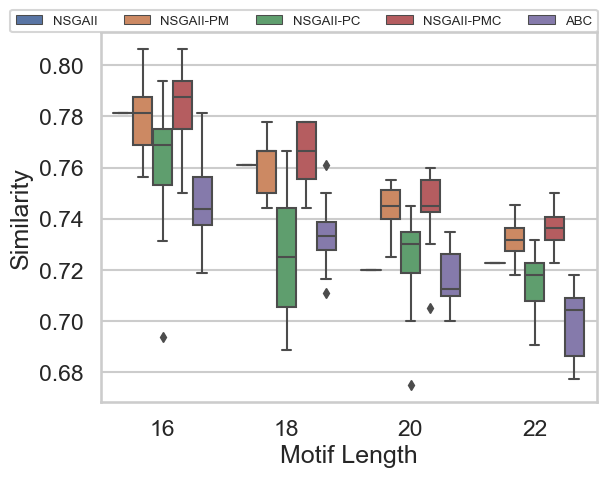
\includegraphics[width=\textwidth]{Figure/hm03_all_boxplot}
			\caption{hm03}
			%\label{fig:con_pr06}
		\end{subfigure}%
		\begin{subfigure}[b]{0.4\textwidth}
			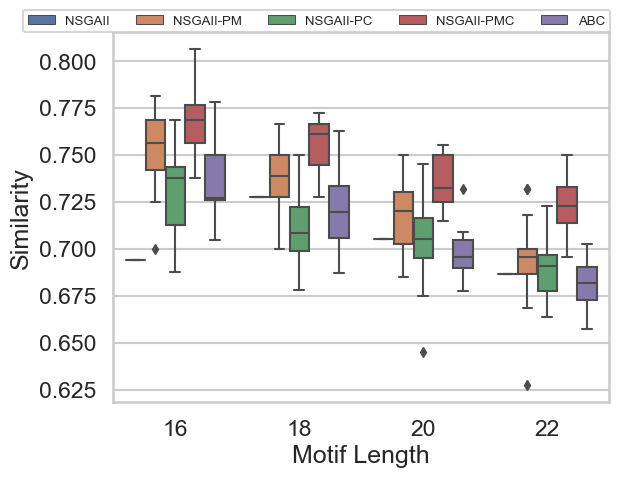
\includegraphics[width=\textwidth]{Figure/hm09g_all_boxplot}
			\caption{hm09g}
			%\label{fig:con_pr07}
		\end{subfigure}%
		\begin{subfigure}[b]{0.4\textwidth}
			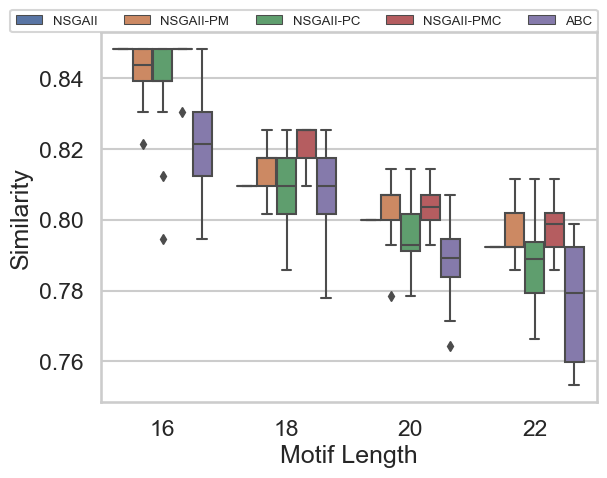
\includegraphics[width=\textwidth]{Figure/yst04r_all_boxplot}
			\caption{yst04r}
			%\label{fig:con_pr09}
		\end{subfigure}    
		\begin{subfigure}[b]{0.4\textwidth}
			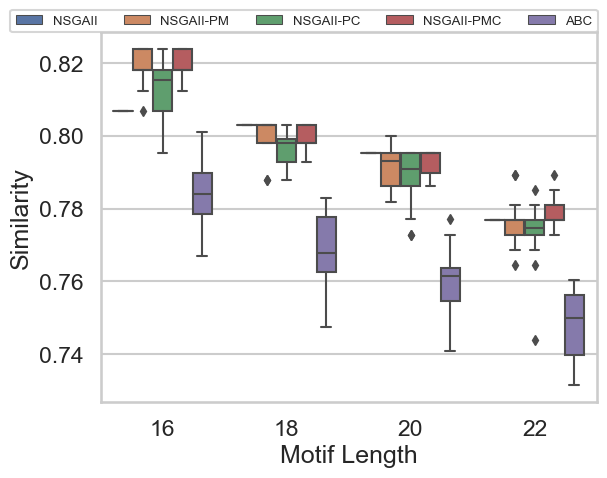
\includegraphics[width=\textwidth]{Figure/yst08r_all_boxplot}
			\caption{yst08r}
			%\label{fig:con_pr06}
		\end{subfigure}%
		\begin{subfigure}[b]{0.4\textwidth}
			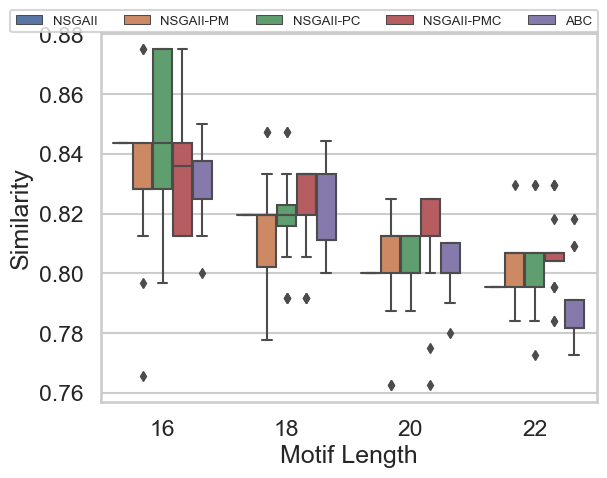
\includegraphics[width=\textwidth]{Figure/dm01g_all_boxplot}
			\caption{dm01g}
			%\label{fig:con_pr07}
		\end{subfigure}%
		\begin{subfigure}[b]{0.4\textwidth}
			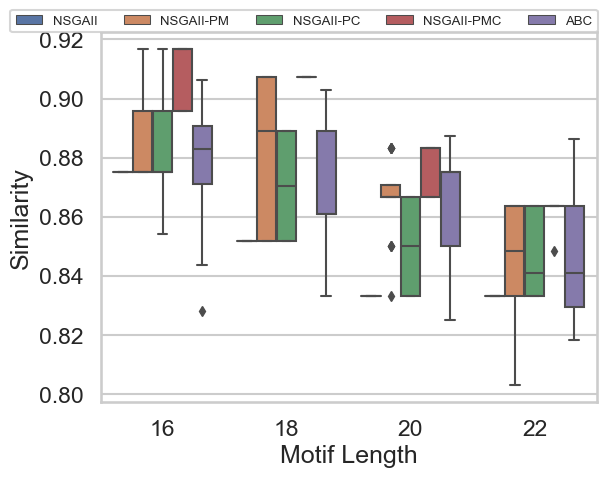
\includegraphics[width=\textwidth]{Figure/dm03g_all_boxplot}
			\caption{dm03g}
			%\label{fig:con_pr09}
		\end{subfigure}
		\caption{Similarity score achieved by ABC and four NSGAII variants on six datasets. }
		\label{fig:gen_wise_correlation}
	\end{adjustwidth}
\end{figure}